% Options for packages loaded elsewhere
\PassOptionsToPackage{unicode}{hyperref}
\PassOptionsToPackage{hyphens}{url}
%
\documentclass[
]{book}
\title{설치형 오픈 통계 패키지 - \texttt{Rcmdr}}
\author{신종화, 이광춘, 유충현, 홍성학}
\date{2022-04-16}

\usepackage{amsmath,amssymb}
\usepackage{lmodern}
\usepackage{iftex}
\ifPDFTeX
  \usepackage[T1]{fontenc}
  \usepackage[utf8]{inputenc}
  \usepackage{textcomp} % provide euro and other symbols
\else % if luatex or xetex
  \usepackage{unicode-math}
  \defaultfontfeatures{Scale=MatchLowercase}
  \defaultfontfeatures[\rmfamily]{Ligatures=TeX,Scale=1}
\fi
% Use upquote if available, for straight quotes in verbatim environments
\IfFileExists{upquote.sty}{\usepackage{upquote}}{}
\IfFileExists{microtype.sty}{% use microtype if available
  \usepackage[]{microtype}
  \UseMicrotypeSet[protrusion]{basicmath} % disable protrusion for tt fonts
}{}
\makeatletter
\@ifundefined{KOMAClassName}{% if non-KOMA class
  \IfFileExists{parskip.sty}{%
    \usepackage{parskip}
  }{% else
    \setlength{\parindent}{0pt}
    \setlength{\parskip}{6pt plus 2pt minus 1pt}}
}{% if KOMA class
  \KOMAoptions{parskip=half}}
\makeatother
\usepackage{xcolor}
\IfFileExists{xurl.sty}{\usepackage{xurl}}{} % add URL line breaks if available
\IfFileExists{bookmark.sty}{\usepackage{bookmark}}{\usepackage{hyperref}}
\hypersetup{
  pdftitle={설치형 오픈 통계 패키지 - Rcmdr},
  pdfauthor={신종화, 이광춘, 유충현, 홍성학},
  hidelinks,
  pdfcreator={LaTeX via pandoc}}
\urlstyle{same} % disable monospaced font for URLs
\usepackage{color}
\usepackage{fancyvrb}
\newcommand{\VerbBar}{|}
\newcommand{\VERB}{\Verb[commandchars=\\\{\}]}
\DefineVerbatimEnvironment{Highlighting}{Verbatim}{commandchars=\\\{\}}
% Add ',fontsize=\small' for more characters per line
\usepackage{framed}
\definecolor{shadecolor}{RGB}{248,248,248}
\newenvironment{Shaded}{\begin{snugshade}}{\end{snugshade}}
\newcommand{\AlertTok}[1]{\textcolor[rgb]{0.94,0.16,0.16}{#1}}
\newcommand{\AnnotationTok}[1]{\textcolor[rgb]{0.56,0.35,0.01}{\textbf{\textit{#1}}}}
\newcommand{\AttributeTok}[1]{\textcolor[rgb]{0.77,0.63,0.00}{#1}}
\newcommand{\BaseNTok}[1]{\textcolor[rgb]{0.00,0.00,0.81}{#1}}
\newcommand{\BuiltInTok}[1]{#1}
\newcommand{\CharTok}[1]{\textcolor[rgb]{0.31,0.60,0.02}{#1}}
\newcommand{\CommentTok}[1]{\textcolor[rgb]{0.56,0.35,0.01}{\textit{#1}}}
\newcommand{\CommentVarTok}[1]{\textcolor[rgb]{0.56,0.35,0.01}{\textbf{\textit{#1}}}}
\newcommand{\ConstantTok}[1]{\textcolor[rgb]{0.00,0.00,0.00}{#1}}
\newcommand{\ControlFlowTok}[1]{\textcolor[rgb]{0.13,0.29,0.53}{\textbf{#1}}}
\newcommand{\DataTypeTok}[1]{\textcolor[rgb]{0.13,0.29,0.53}{#1}}
\newcommand{\DecValTok}[1]{\textcolor[rgb]{0.00,0.00,0.81}{#1}}
\newcommand{\DocumentationTok}[1]{\textcolor[rgb]{0.56,0.35,0.01}{\textbf{\textit{#1}}}}
\newcommand{\ErrorTok}[1]{\textcolor[rgb]{0.64,0.00,0.00}{\textbf{#1}}}
\newcommand{\ExtensionTok}[1]{#1}
\newcommand{\FloatTok}[1]{\textcolor[rgb]{0.00,0.00,0.81}{#1}}
\newcommand{\FunctionTok}[1]{\textcolor[rgb]{0.00,0.00,0.00}{#1}}
\newcommand{\ImportTok}[1]{#1}
\newcommand{\InformationTok}[1]{\textcolor[rgb]{0.56,0.35,0.01}{\textbf{\textit{#1}}}}
\newcommand{\KeywordTok}[1]{\textcolor[rgb]{0.13,0.29,0.53}{\textbf{#1}}}
\newcommand{\NormalTok}[1]{#1}
\newcommand{\OperatorTok}[1]{\textcolor[rgb]{0.81,0.36,0.00}{\textbf{#1}}}
\newcommand{\OtherTok}[1]{\textcolor[rgb]{0.56,0.35,0.01}{#1}}
\newcommand{\PreprocessorTok}[1]{\textcolor[rgb]{0.56,0.35,0.01}{\textit{#1}}}
\newcommand{\RegionMarkerTok}[1]{#1}
\newcommand{\SpecialCharTok}[1]{\textcolor[rgb]{0.00,0.00,0.00}{#1}}
\newcommand{\SpecialStringTok}[1]{\textcolor[rgb]{0.31,0.60,0.02}{#1}}
\newcommand{\StringTok}[1]{\textcolor[rgb]{0.31,0.60,0.02}{#1}}
\newcommand{\VariableTok}[1]{\textcolor[rgb]{0.00,0.00,0.00}{#1}}
\newcommand{\VerbatimStringTok}[1]{\textcolor[rgb]{0.31,0.60,0.02}{#1}}
\newcommand{\WarningTok}[1]{\textcolor[rgb]{0.56,0.35,0.01}{\textbf{\textit{#1}}}}
\usepackage{longtable,booktabs,array}
\usepackage{calc} % for calculating minipage widths
% Correct order of tables after \paragraph or \subparagraph
\usepackage{etoolbox}
\makeatletter
\patchcmd\longtable{\par}{\if@noskipsec\mbox{}\fi\par}{}{}
\makeatother
% Allow footnotes in longtable head/foot
\IfFileExists{footnotehyper.sty}{\usepackage{footnotehyper}}{\usepackage{footnote}}
\makesavenoteenv{longtable}
\usepackage{graphicx}
\makeatletter
\def\maxwidth{\ifdim\Gin@nat@width>\linewidth\linewidth\else\Gin@nat@width\fi}
\def\maxheight{\ifdim\Gin@nat@height>\textheight\textheight\else\Gin@nat@height\fi}
\makeatother
% Scale images if necessary, so that they will not overflow the page
% margins by default, and it is still possible to overwrite the defaults
% using explicit options in \includegraphics[width, height, ...]{}
\setkeys{Gin}{width=\maxwidth,height=\maxheight,keepaspectratio}
% Set default figure placement to htbp
\makeatletter
\def\fps@figure{htbp}
\makeatother
\setlength{\emergencystretch}{3em} % prevent overfull lines
\providecommand{\tightlist}{%
  \setlength{\itemsep}{0pt}\setlength{\parskip}{0pt}}
\setcounter{secnumdepth}{5}
\usepackage{booktabs}
\usepackage{amsthm}
\makeatletter
\def\thm@space@setup{%
  \thm@preskip=8pt plus 2pt minus 4pt
  \thm@postskip=\thm@preskip
}
\makeatother
\ifLuaTeX
  \usepackage{selnolig}  % disable illegal ligatures
\fi
\usepackage[]{natbib}
\bibliographystyle{apalike}

\begin{document}
\maketitle

{
\setcounter{tocdepth}{1}
\tableofcontents
}
\hypertarget{uxb4e4uxc5b4uxac00uxba70}{%
\chapter{들어가며}\label{uxb4e4uxc5b4uxac00uxba70}}

\textbf{한국 알(R) 사용자회}는 디지털 불평등 해소와 통계 대중화를 오픈 통계 패키지 개발을 2021년부터 추진하였습니다.
더불어 설치형 오픈 통계 패키지를 신종화 님께서 John Fox 교수님이 개발한 \texttt{Rcmdr} 기반으로 한글화 및 문서화에 10년 넘게 기여해주셨습니다. 이에 \textbf{한국 알(R) 사용자회}는 신종화님의 \texttt{Rcmdr} 거인의 어깨위에 디지털 불평등 해소와 통계 대중화를 위해 한 걸음 더 나아가게 되었습니다. 특히 신종화님께서 기여하신 한글화 및 문서를 근간으로 더 많은 분들이 오픈 통계 패키지를 사용할 수 있도록 \texttt{bookdown}으로 내용을 정리하여 통계 대중화가 한층 앞당겨질 것으로 기대됩니다.

신종화님께서 왜 오픈 통계 패키지로 \texttt{Rcmdr}를 근간으로 해야 하는지 이유를 명쾌하게 다음과 같이 정리해 주셨습니다.

R에는 여러 개의 GUI 작업도구들이 있습니다. 모두 목적이 분명하고, 좋은 도구이며, 일부는 현재도 향상작업이 진행되고 있습니다. 그럼에도 불구하고 R Commander를 위한 블로그 작업을 진행하는 이유는 크게 두가지 입니다.

첫째, R Commander는 직관적으로 기존의 기초통계학 도구와 유사합니다. Command Line 에서 작업하는 것에 익숙하지 않은, 또 어려움을 겪고 있는 사용자들에게 기초통계학분야를 학습하고 활용하는데 도움을 주기 위하여 R Commander가 개발되었습니다. 개발자인 John Fox 교수는 이 목적과 관리방향을 분명히하고 있습니다. 중급이상의 R 사용자/ 고급통계 연구자들에게는 R Commander가 불필요할 수 있습니다.

둘째, 지난 10년동안 R Commander의 메뉴 한글화작업을 진행해왔으며, 현재도 유지관리를 하고 있습니다. (이 정보는 R Commander 안의 Help \textgreater{} About Rcmdr 에 있습니다) {[}Translations: Korean, Chel Hee Lee, Dae-Heung Jang, and Shin Jong-Hwa{]} 지난 10년 동안 개인적인 메모 차원에서 R Commander 사용 및 한글화 관련 블로그 포스트를 만들고 관리되어 왔고 \href{http://modernity.tistory.com}{블로그}에 전체 과정이 고스란히 남아있고 계속적으로 유지관리될 것입니다.

\begin{itemize}
\tightlist
\item
  신종화 \href{https://rcmdr.kr/}{Rcmdr : R Commander}
\item
  \href{https://cran.r-project.org/web/packages/Rcmdr/index.html}{CRAN Rcmdr 패키지 정보}
\item
  \href{https://socialsciences.mcmaster.ca/jfox/Misc/Rcmdr/}{개발자 John Fox 교수의 Rcmdr 소개}
\item
  \href{https://modernity.tistory.com/}{FOSSER\_Ricoop}
\end{itemize}

\hypertarget{install}{%
\chapter{설치}\label{install}}

\hypertarget{uxb3c4uxc6c0uxb9d0-help}{%
\chapter{\texorpdfstring{도움말 / \texttt{Help}}{도움말 / Help}}\label{uxb3c4uxc6c0uxb9d0-help}}

\hypertarget{commander-help-0}{%
\section{Commander help (0)}\label{commander-help-0}}

\hypertarget{introduction-to-the-r-comma..-0}{%
\section{Introduction to the R Comma.. (0)}\label{introduction-to-the-r-comma..-0}}

\hypertarget{r-commander-website-0}{%
\section{R Commander website (0)}\label{r-commander-website-0}}

\hypertarget{about-rcmdr-0}{%
\section{About Rcmdr (0)}\label{about-rcmdr-0}}

\hypertarget{r-commander-hex-sticker}{%
\section{R Commander hex sticker}\label{r-commander-hex-sticker}}

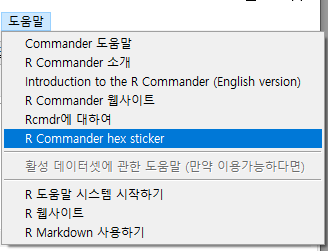
\includegraphics{fig/help-01.png}

선택하면 아래와 같은 이미지 파일이 등장한다:


\includegraphics{fig/help-02.png}

\hypertarget{help-on-active-data-set-if..-0}{%
\section{Help on active data set (if.. (0)}\label{help-on-active-data-set-if..-0}}

\hypertarget{start-r-help-system-0}{%
\section{Start R help system (0)}\label{start-r-help-system-0}}

\hypertarget{r-website-0}{%
\section{R website (0)}\label{r-website-0}}

\hypertarget{using-r-markdown-0}{%
\section{Using R Markdown (0)}\label{using-r-markdown-0}}

\hypertarget{uxb370uxc774uxd130uxc14b-datasets}{%
\chapter{\texorpdfstring{데이터셋 / \texttt{datasets}}{데이터셋 / datasets}}\label{uxb370uxc774uxd130uxc14b-datasets}}

\hypertarget{prestige---cardata-prestige}{%
\section{\texorpdfstring{Prestige - \texttt{carData\ \textgreater{}\ Prestige}}{Prestige - carData \textgreater{} Prestige}}\label{prestige---cardata-prestige}}

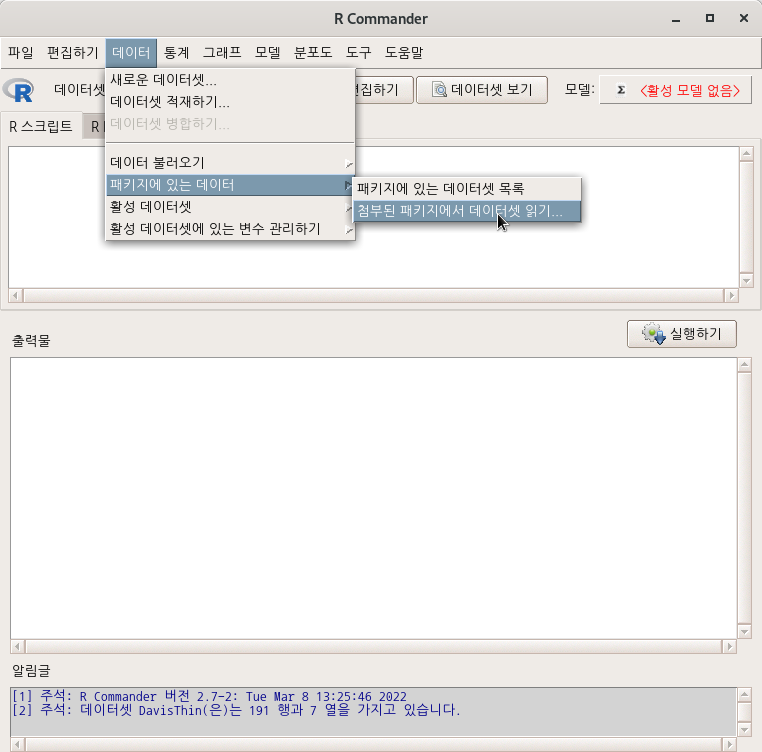
\includegraphics{fig/dataset-prestiage-01.png}

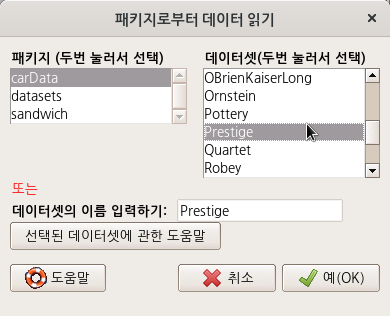
\includegraphics{fig/dataset-prestiage-02.png}

\begin{Shaded}
\begin{Highlighting}[]
\FunctionTok{data}\NormalTok{(Prestige, }\AttributeTok{package=}\StringTok{"carData"}\NormalTok{)}
\end{Highlighting}
\end{Shaded}

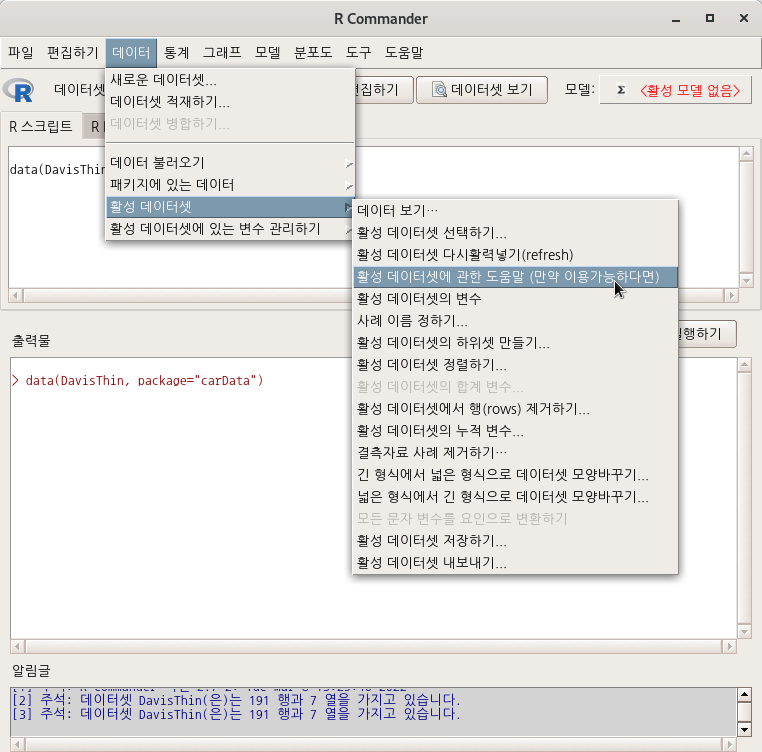
\includegraphics{fig/dataset-prestiage-03.png}

\begin{Shaded}
\begin{Highlighting}[]
\FunctionTok{help}\NormalTok{(}\StringTok{"Prestige"}\NormalTok{)}
\end{Highlighting}
\end{Shaded}

carData 패키지에 있는 Prestige 데이터셋을 \texttt{.csv}로 저장하여 내보낼 수 있다.

\href{data/Prestige.csv}{다운로드}

참조: \href{https://rcmdr.tistory.com/52}{활성 데이터셋 내보내기\ldots{}}

\hypertarget{moore---cardata-moore}{%
\section{\texorpdfstring{Moore - \texttt{carData\ \textgreater{}\ Moore}}{Moore - carData \textgreater{} Moore}}\label{moore---cardata-moore}}

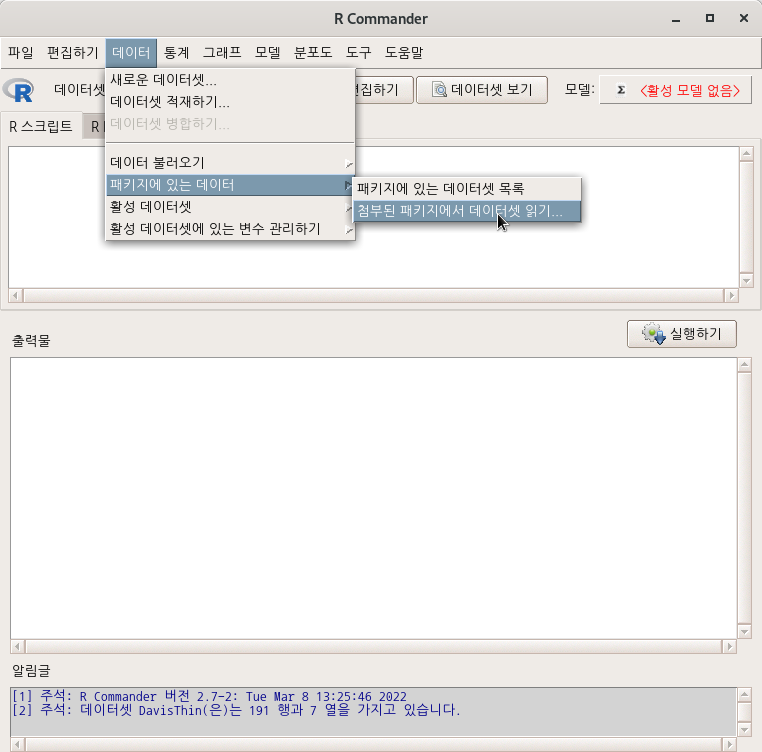
\includegraphics{fig/dataset-moore-01.png}

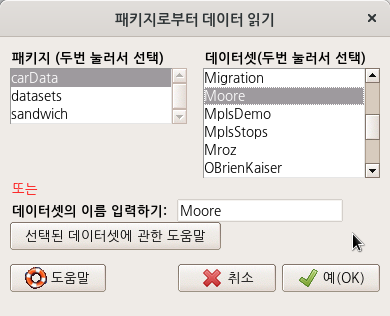
\includegraphics{fig/dataset-moore-02.png}

\begin{Shaded}
\begin{Highlighting}[]
\FunctionTok{data}\NormalTok{(Moore, }\AttributeTok{package=}\StringTok{"carData"}\NormalTok{)}
\end{Highlighting}
\end{Shaded}

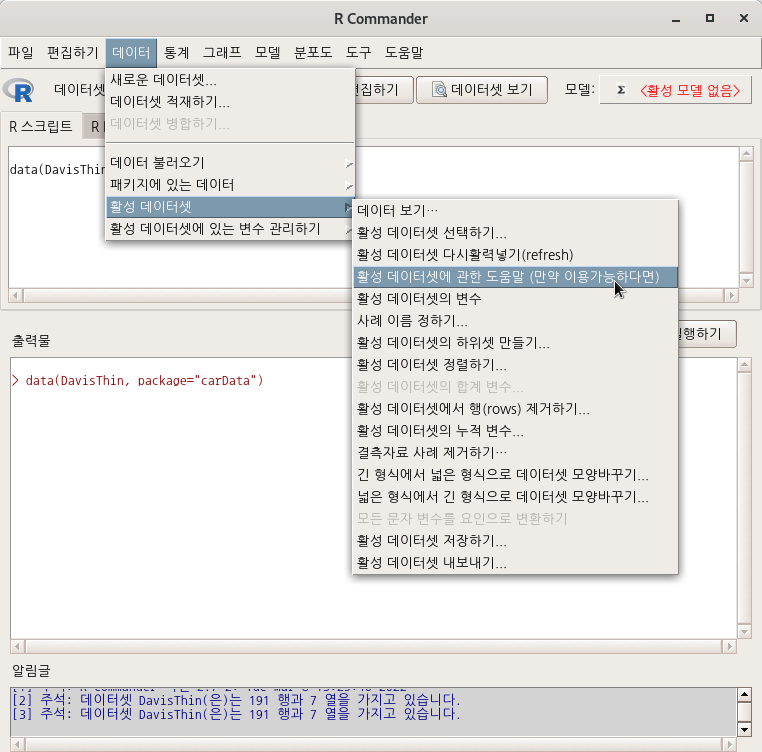
\includegraphics{fig/dataset-moore-03.png}

\begin{Shaded}
\begin{Highlighting}[]
\FunctionTok{help}\NormalTok{(}\StringTok{"Moore"}\NormalTok{)}
\end{Highlighting}
\end{Shaded}

상기 명령 실행을 통해서 \texttt{Moore} 데이터셋에 대한 상세 정보를 얻을 수 있다.

Moore \{carData\}

R Documentation

Status, Authoritarianism, and Conformity

Description

The Moore data frame has 45 rows and 4 columns.
The data are for subjects in a social-psychological experiment,
who were faced with manipulated disagreement from a partner of either
of low or high status. The subjects could either conform to the
partner's judgment or stick with their own judgment.

Usage

Format

This data frame contains the following columns:

partner.status

Partner's status. A factor with levels:
high,
low.

conformity

Number of conforming responses in 40 critical trials.

fcategory

F-Scale Categorized.
A factor with levels (note levels out of order):
high,
low,
medium.

fscore

Authoritarianism: F-Scale score.

Source

Moore, J. C., Jr.~and Krupat, E. (1971)
Relationship between source status, authoritarianism and conformity in a
social setting. Sociometry 34, 122--134.

Personal communication
from J. Moore, Department of Sociology, York University.

References

Fox, J. (2016)
Applied Regression Analysis and Generalized Linear Models,
Third Edition. Sage.

Fox, J. and Weisberg, S. (2019)
An R Companion to Applied Regression, Third Edition, Sage.

{[}Package carData version 3.0-5 Index{]}

\hypertarget{obrienkaiser---cardata-obrienkaiser}{%
\section{\texorpdfstring{OBrienKaiser - \texttt{carData\ \textgreater{}\ OBrienKaiser}}{OBrienKaiser - carData \textgreater{} OBrienKaiser}}\label{obrienkaiser---cardata-obrienkaiser}}

\texttt{carData} 패키지에 있는 \texttt{OBrienKaiser} 데이터셋이다. \texttt{carData} 패키지는 \texttt{Rcmdr} 패키지가 호출될 때 자동으로 함께 호출되기 때문에 \textbf{R Commander}에서 \texttt{carData} 패키지에 포함된 데이터셋들을 자유롭게 호출할 수 있다.

\href{https://rcmdr.kr/37}{Read data set from an attached package\ldots{}}

OBrienKaiser 데이터셋은 R Commander에서 활성 데이터셋으로 이용할 수 있다. 그러나 `통계 \textgreater{} 요약 \textgreater{} 활성데이터셋' 기능은 사용할 수 없다. 다음과 같은 오류문을 Rgui 창에서 보게된다.

\begin{quote}
Error in sprintf(gettextRcmdr(``There are \%d variables in the data set \%s.\nDo you want to proceed?''), :
'\%d'는 유효하지 않은 포맷입니다; 문자형 객체들에는 포맷 \%s를 사용해주세요
\end{quote}

입력창에 str(OBrienKaiser) 함수를 입력하고 실행하여 OBrienKaiser 데이터셋의 구조를 살펴보자.

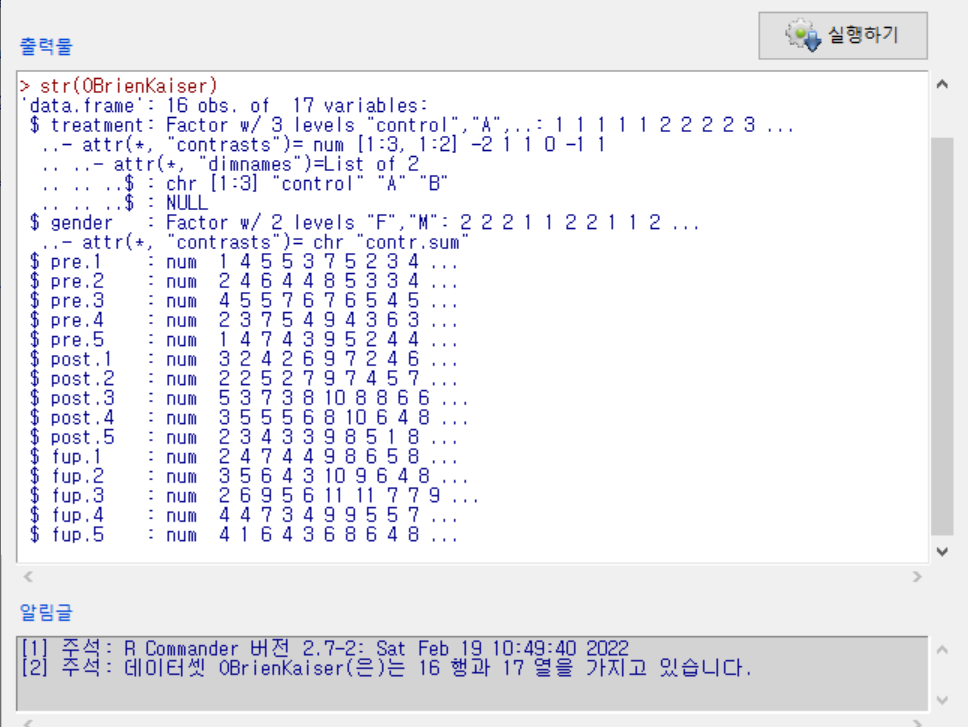
\includegraphics{fig/dataset-obrien-01.png}

입력창에 \texttt{summary(OBrienKaiser)} 함수를 입력하고 실행하여 요약 정보를 살펴보자.

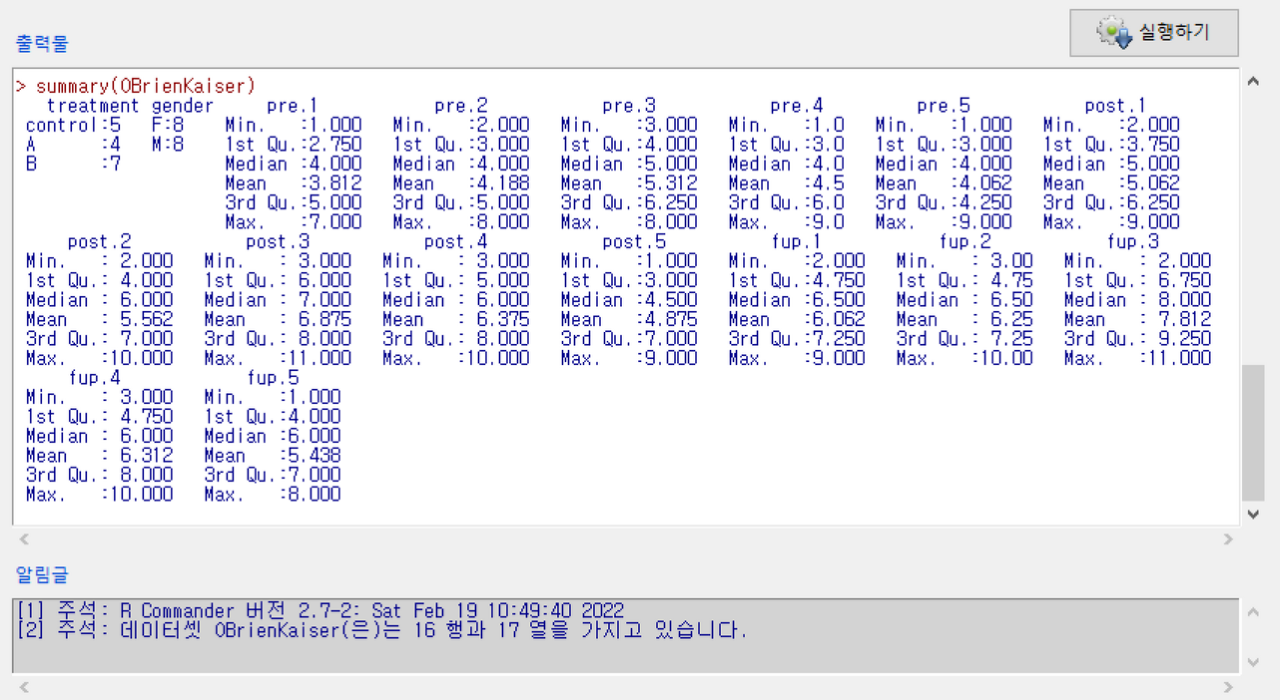
\includegraphics{fig/dataset-obrien-02.png}

OBrienKaiser \{carData\}

R Documentation

O'Brien and Kaiser's Repeated-Measures Data

Description

These contrived repeated-measures data are taken from
O'Brien and Kaiser (1985). The data are from an imaginary study in which
16 female and male subjects, who are divided into three treatments, are measured
at a pretest, postest, and a follow-up session; during each session, they are
measured at five occasions at intervals of one hour. The design, therefore, has
two between-subject and two within-subject factors.

The contrasts for the treatment factor are set to -2, 1, 1 and
0, -1, 1. The contrasts for the gender factor are set to
contr.sum.

Usage

Format

A data frame with 16 observations on the following 17 variables.

treatment

a factor with levels control A B

gender

a factor with levels F M

pre.1

pretest, hour 1

pre.2

pretest, hour 2

pre.3

pretest, hour 3

pre.4

pretest, hour 4

pre.5

pretest, hour 5

post.1

posttest, hour 1

post.2

posttest, hour 2

post.3

posttest, hour 3

post.4

posttest, hour 4

post.5

posttest, hour 5

fup.1

follow-up, hour 1

fup.2

follow-up, hour 2

fup.3

follow-up, hour 3

fup.4

follow-up, hour 4

fup.5

follow-up, hour 5

Source

O'Brien, R. G., and Kaiser, M. K. (1985)
MANOVA method for analyzing repeated measures designs: An extensive primer.
Psychological Bulletin 97, 316--333, Table 7.

Examples

{[}Package carData version 3.0-5 Index{]}

\hypertarget{obrienkaiserlong---cardata-obrienkaiserlong}{%
\section{\texorpdfstring{OBrienKaiserLong - \texttt{carData\ \textgreater{}\ OBrienKaiserLong}}{OBrienKaiserLong - carData \textgreater{} OBrienKaiserLong}}\label{obrienkaiserlong---cardata-obrienkaiserlong}}

\texttt{OBrienKaiserLong} 데이터셋은 \texttt{carData} 패키지에 포함되어 있다.
\texttt{carData} 패키지는 \texttt{Rcmdr} 패키지가 호출될 때 자동으로 함께 호출되기 때문에, \texttt{OBrienKaiserLong} 데이터셋을 R Commander에서 메뉴기능을 통해서 활성데이터셋으로 불러올 수 있다.

통계\textgreater{} 요약 \textgreater{} 활성 데이터셋 메뉴를 통하여 OBrienKaiserLong 데이터셋의 요약정보를 확인할 수 있다.

\begin{figure}
\centering
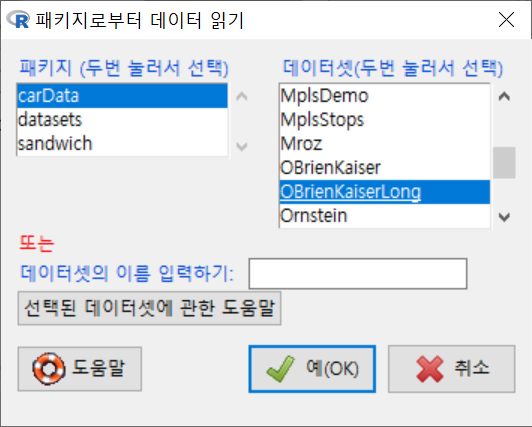
\includegraphics{fig/dataset-obrienlong-01.png}
\caption{Windows 사례}
\end{figure}

\texttt{summary()} 함수를 이용한 것을 알 수 있다.

\begin{figure}
\centering
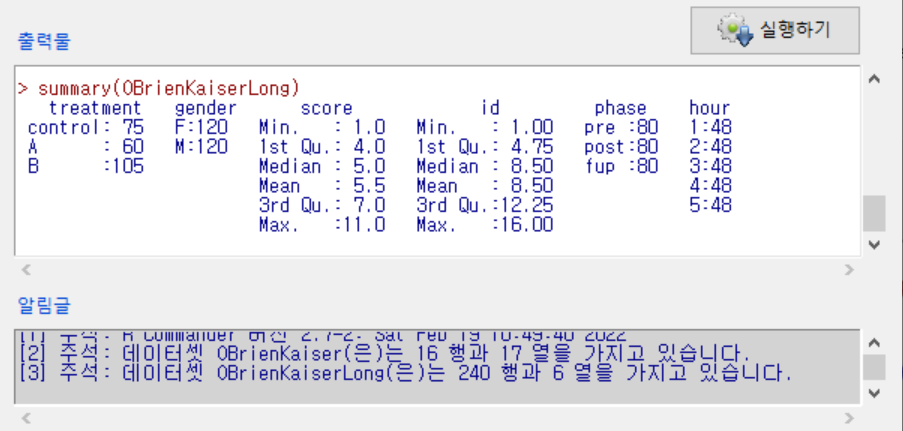
\includegraphics{fig/dataset-obrienlong-02.png}
\caption{Windows 사례}
\end{figure}

\texttt{str()} 함수를 활용하여 입력창에 직접 \texttt{str(OBrienKaiserLong)}을 입력하고 실행하여, 출력창에 다음과 같이 \texttt{OBrienKaiserLong} 데이터셋의 구조적 정보도 확인할 수 있다.

\begin{figure}
\centering
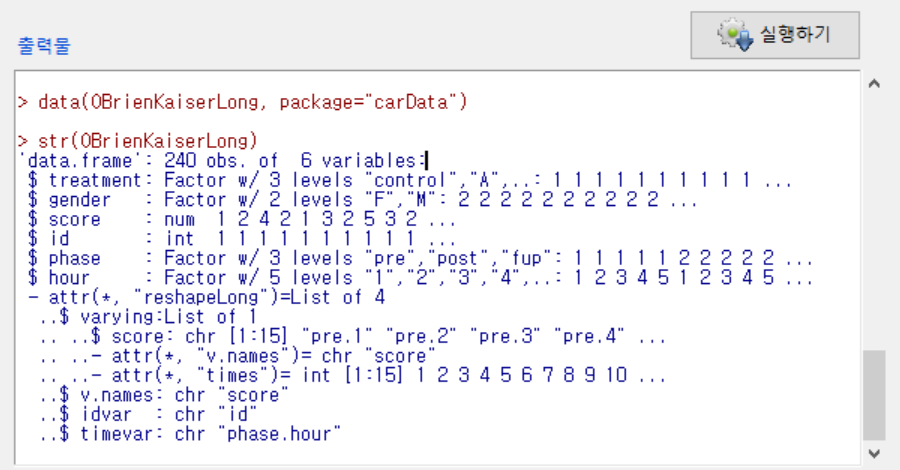
\includegraphics{fig/dataset-obrienlong-03.png}
\caption{Windows 사례}
\end{figure}

R Commander 화면에서 버튼을 누르면 다음과 같은 내부 구성을 볼 수 있다:

\begin{figure}
\centering
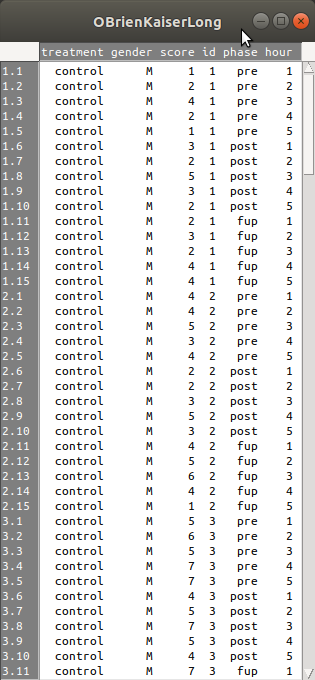
\includegraphics{fig/dataset-obrienlong-04.png}
\caption{Linux 사례 (Ubuntu 18.04)}
\end{figure}

\begin{Shaded}
\begin{Highlighting}[]
\FunctionTok{head}\NormalTok{(OBrienKaiserLong, }\DecValTok{1}\NormalTok{) }\CommentTok{\# first subject}
\end{Highlighting}
\end{Shaded}

OBrienKaiserLong \{carData\}

R Documentation

O'Brien and Kaiser's Repeated-Measures Data in "Long" Format

Description

Contrived repeated-measures data from O'Brien and Kaiser (1985). For details see OBrienKaiser, which is for the "wide" form of the same data.

Usage

Format

A data frame with 240 observations on the following 6 variables.

treatment

a between-subjects factor with levels control, A, B.

gender

a between-subjects factor with levels F, M.

score

the numeric response variable.

id

the subject id number.

phase

a within-subjects factor with levels pre, post, fup.

hour

a within-subjects factor with levels 1, 2, 3, 4, 5.

Source

O'Brien, R. G., and Kaiser, M. K. (1985)
MANOVA method for analyzing repeated measures designs: An extensive primer.
Psychological Bulletin 97, 316--333, Table 7.

See Also

OBrienKaiser.

Examples

{[}Package carData version 3.0-5 Index{]}

\hypertarget{airquality---datasets-airquality}{%
\section{\texorpdfstring{airquality - \texttt{datasets\ \textgreater{}\ airquality}}{airquality - datasets \textgreater{} airquality}}\label{airquality---datasets-airquality}}

\begin{figure}
\centering
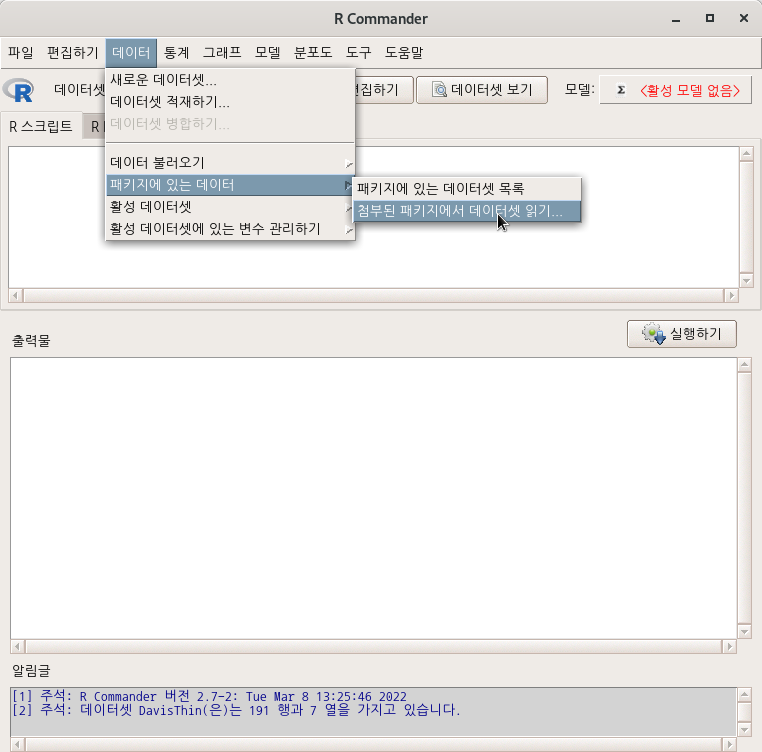
\includegraphics{fig/dataset-airquality-01.png}
\caption{Linux 사례 (MX 21)}
\end{figure}

R이 시작될 때, datasets 패키지가 자동으로 호출된다. 따라서 R Commander를 실행할 때, datasets 패키지는 첨부 패키지화되어 메뉴창을 통해서 내부 데이터셋을 찾고 불러올 수 있다.

메뉴창에서 순서대로 데이터 \textgreater{} 패키지에 있는 데이터 \textgreater{} 첨부된 패키지에서 데이터셋 읽기\ldots{} 를 선택하면 다음과 같은 창이 등장한다.

\begin{figure}
\centering
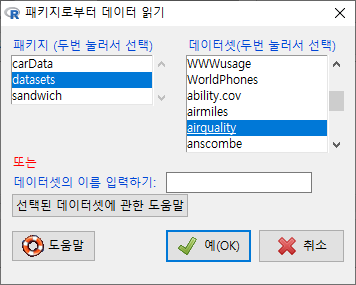
\includegraphics{fig/dataset-airquality-02.png}
\caption{Windows 사례}
\end{figure}

출력창을 보면, airquality라는 데이터셋에는 6개의 변수가 있고, 각 변수는 수치형 정보를 담고 있다.

\begin{figure}
\centering
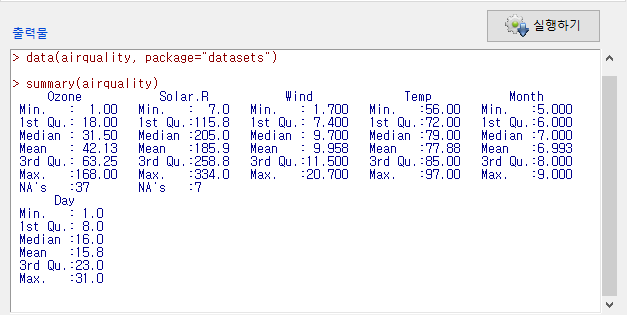
\includegraphics{fig/dataset-airquality-03.png}
\caption{Windows 사례}
\end{figure}

Month 변수는 최소 5에서 최대 9로 값이 있는데, 정확히는 5월부터 9월까지일 것이다. 한달 한달을 뜻하는 월(month)은 5월이 9월보다 크다고 할 수 없고, 5월, 6월, 7월, 8월, 9월 등으로 개체화되어 분리된다. 다시 말하면, 요인형 변수가 되어야 한다는 뜻이다.

그럼 왜, airqualty 데이터셋의 Month 변수는 수치형으로 되어 있을까. 원자료를 R의 데이터셋으로 불러오는 과정에서 해당 변수의 요인화과정이 생략되었을 것이다.

airquality \{datasets\}

R Documentation

New York Air Quality Measurements

Description

Daily air quality measurements in New York, May to September 1973.

Usage

Format

A data frame with 153 observations on 6 variables.

{[},1{]}

Ozone

numeric

Ozone (ppb)

{[},2{]}

Solar.R

numeric

Solar R (lang)

{[},3{]}

Wind

numeric

Wind (mph)

{[},4{]}

Temp

numeric

Temperature (degrees F)

{[},5{]}

Month

numeric

Month (1--12)

{[},6{]}

Day

numeric

Day of month (1--31)

Details

Daily readings of the following air quality values for May 1, 1973 (a
Tuesday) to September 30, 1973.

Ozone: Mean ozone in parts per
billion from 1300 to 1500 hours at Roosevelt Island

Solar.R: Solar radiation
in Langleys in the frequency band 4000--7700 Angstroms from
0800 to 1200 hours at Central Park

Wind: Average wind speed in miles
per hour at 0700 and 1000 hours at LaGuardia Airport

Temp: Maximum daily
temperature in degrees Fahrenheit at La Guardia Airport.

Source

The data were obtained from the New York State Department of
Conservation (ozone data) and the National Weather Service
(meteorological data).

References

Chambers, J. M., Cleveland, W. S., Kleiner, B. and Tukey, P. A. (1983)
Graphical Methods for Data Analysis.
Belmont, CA: Wadsworth.

Examples

{[}Package datasets version 4.1.3 Index{]}

\hypertarget{bfox}{%
\section{Bfox}\label{bfox}}

\hypertarget{sleep-1}{%
\section{sleep (1)}\label{sleep-1}}

\hypertarget{davisthin-1}{%
\section{DavisThin (1)}\label{davisthin-1}}

\hypertarget{usarrests-1}{%
\section{USArrests (1)}\label{usarrests-1}}

\hypertarget{birthwt-1}{%
\section{birthwt (1)}\label{birthwt-1}}

\hypertarget{friendly-1}{%
\section{Friendly (1)}\label{friendly-1}}

\hypertarget{cowles-1}{%
\section{Cowles (1)}\label{cowles-1}}

\hypertarget{adler-1}{%
\section{Adler (1)}\label{adler-1}}

\hypertarget{warpbreaks-1}{%
\section{warpbreaks (1)}\label{warpbreaks-1}}

  \bibliography{book.bib,packages.bib}

\end{document}
